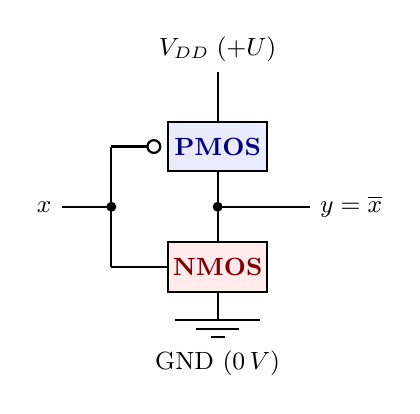
\begin{tikzpicture}[scale=0.9, >=stealth]
    % Versorgung oben (VDD)
    \draw[thick] (2,3.1) node[above, font=\small] {$V_{DD} \; (+U)$} -- (2,2.4);

    % PMOS oben (p-Kanal Transistor)
    \draw[thick, fill=blue!8] (1.3,1.7) rectangle (2.7,2.4);
    \node[font=\small\bfseries, color=NavyBlue] at (2,2.05) {PMOS};
    \draw[thick] (1.1,2.05) circle (0.09cm); % Invertierungskreis
    \draw[thick] (0.5,2.05) -- (1.01,2.05);

    % Verbindung zwischen PMOS und NMOS
    \draw[thick] (2,1.7) -- (2,0.7);
    \draw[thick] (2,1.2) -- (3.3,1.2) node[right, font=\small] {$y = \overline{x}$};
    \fill (2,1.2) circle (2pt);

    % NMOS unten (n-Kanal Transistor)
    \draw[thick, fill=red!8] (1.3,0) rectangle (2.7,0.7);
    \node[font=\small\bfseries, color=Maroon] at (2,0.35) {NMOS};
    \draw[thick] (0.5,0.35) -- (1.3,0.35);

    % Masse unten (GND)
    \draw[thick] (2,0) -- (2,-0.4);
    \draw[thick] (1.4,-0.4) -- (2.6,-0.4);
    \draw[thick] (1.7,-0.52) -- (2.3,-0.52);
    \draw[thick] (1.9,-0.64) -- (2.1,-0.64);
    \node[below, font=\small] at (2,-0.7) {GND ($0\,\text{V}$)};

    % Eingang x
    \draw[thick] (0.5,2.05) -- (0.5,0.35);
    \draw[thick] (-0.2,1.2) node[left, font=\small] {$x$} -- (0.5,1.2);
    \fill (0.5,1.2) circle (2pt);
\end{tikzpicture}
